\section{Repositories}
To ensure that the system is not hard-coded to fit unto a specific database system, the repository pattern \citep{RepositoryPattern} has been used to ensure the possibility of changing the database structure at a later date, without re-coding the core functionality. The repository pattern is used to create a uniform interface, connecting the database to the rest of the system. As long as any database access implementation depends on the repository-interfaces, it can connect to any version of any database system.
\par
The repository pattern encapsulates the functionality of creating, updating, reading, and removing data within the database, so it decouples this functionality, from the core of the system. 
\par
This implementation has been a focus area, to make it easier for Aalborg Zoo to move to another database structure or platform at a later date, if necessary. 

\begin{figure}[H]
    \centering
    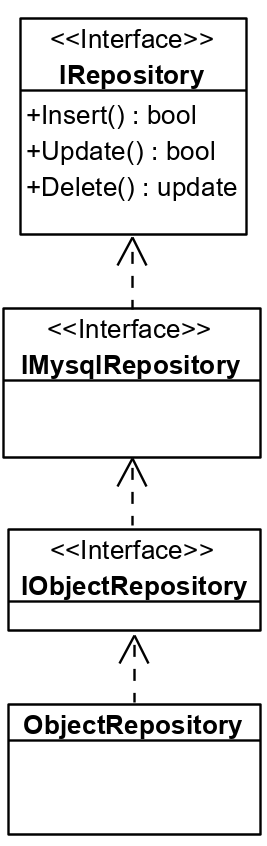
\includegraphics[width=0.2\textwidth]{figures/Implementation/GenericRepositoryStructure.PNG}
    \caption{\textbf{PLACEHOLDER} repository diagram}
    \label{fig:RepositoryDiagram}
\end{figure}

The system specific structure of the implementation can be seen on \autoref{fig:RepositoryDiagram}.
\par
Any database access implemented by the system needs to implement the different interfaces. As seen in \autoref{fig:RepositoryDiagram} all of the database related repositories depend on \textit{IRepository}. This is done to ensure that the database interfaces implement \textbf{\textit{Insert()}}, \textbf{\textit{Update()}} and \textbf{\textit{Delete()}} as functions. By implementing these interfaces the database access implementation, satisfies the general needs for database access implementations.
\par
Depending on which repository is used (\textit{Asset}, \textit{Log}, \textit{Tag}, etc.) different functionalities needs to be implemented.
The interfaces on the third layer of \autoref{fig:RepositoryDiagram} define the functionalities specific to the objects, which the individual repository classes should implement. These classes handle the connections to the database, and handle the SQL scripts to the database, as well as constructing these scripts to fit to the specific model. 
\par
As some of the models have unique ways of being searched/added/edited in the database, individual interfaces were needed for these, to make sure the objects were saved and loaded correctly. 
\\
At the bottom of \autoref{fig:RepositoryDiagram}, the object repository is defined. This class contains all the information and functions related to a specific model, defined in the chain of interfaces.
\\
If a new database structure where to be added at a later date, it would just have to define a dependency to the last of the "ObjectRepository", and will hereby be forced to implement the required functions, to make the database connection useful.
